%
% fig-sinxx.tex
%
% (c) 2026 Prof Dr Andreas Müller
%
\begin{figure}
\centering
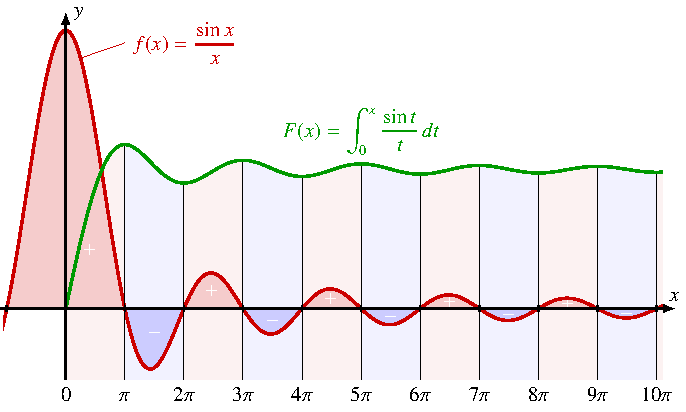
\includegraphics{chapters/030-integration/images/sinxx.pdf}
\caption{Die Stammfunktion von $f(x) = \sin(x)/x$ oszilliert, die Extrema
befinden sich bei den Nullstellen des Integranden, die ganzzahlige
Vielfache von $\pi$ sind.
\label{buch:integration:fig:sinxx}}
\end{figure}
